\documentclass[11pt]{amsart}
\usepackage{geometry}                % See geometry.pdf to learn the layout options. There are lots.
\geometry{letterpaper}                   % ... or a4paper or a5paper or ... 
%\geometry{landscape}                % Activate for for rotated page geometry
%\usepackage[parfill]{parskip}    % Activate to begin paragraphs with an empty line rather than an indent
\usepackage{graphicx}
\usepackage{amssymb}
\usepackage{epstopdf}
\DeclareGraphicsRule{.tif}{png}{.png}{`convert #1 `dirname #1`/`basename #1 .tif`.png}

\title{Inquiryweb Design Document}
\author{John Burk}
%\date{}                                           % Activate to display a given date or no date

\begin{document}
\maketitle
\section{Purpose/Problem}
The process of inquiry in the science classroom is messy. Teachers and students ask questions, make observations, collect evidence, offer explanations and build models throughout the process of learning. Great scientists tell us that the science questions only lead to more questions. What if there were an easy way to track this inquiry process in the moment�as a student asks a question or right as she is taking data? What if other students could browse the questions, evidence and conclusion and see how they are linked together into a web of understanding? 

Inquiryweb is designed to simplify this process of inquiry by keeping track of all of the questions, evidence, conclusions, observations that arise in the classroom, in the moment, with minimal overhead. Asking a question, tagging it, and linking it to other questions is a simple process designed for quick entry by students or faculty. 

Inquiryweb should allow users to quickly enter events (questions, observations, conclusions, and answers) and then link those events to other events in the knowledge web the class generated. Events can then be browsed, and searched, so that students can traverse the class's path of understanding, search our unanswered questions, or connect observations into an explanation. 

Teachers too can search and browse the the knowedlgeweb, along with statistics summarizing each studnets' contributions to the inquiryweb. 


\section{Design}

\begin{figure}[htbp]
   \centering
   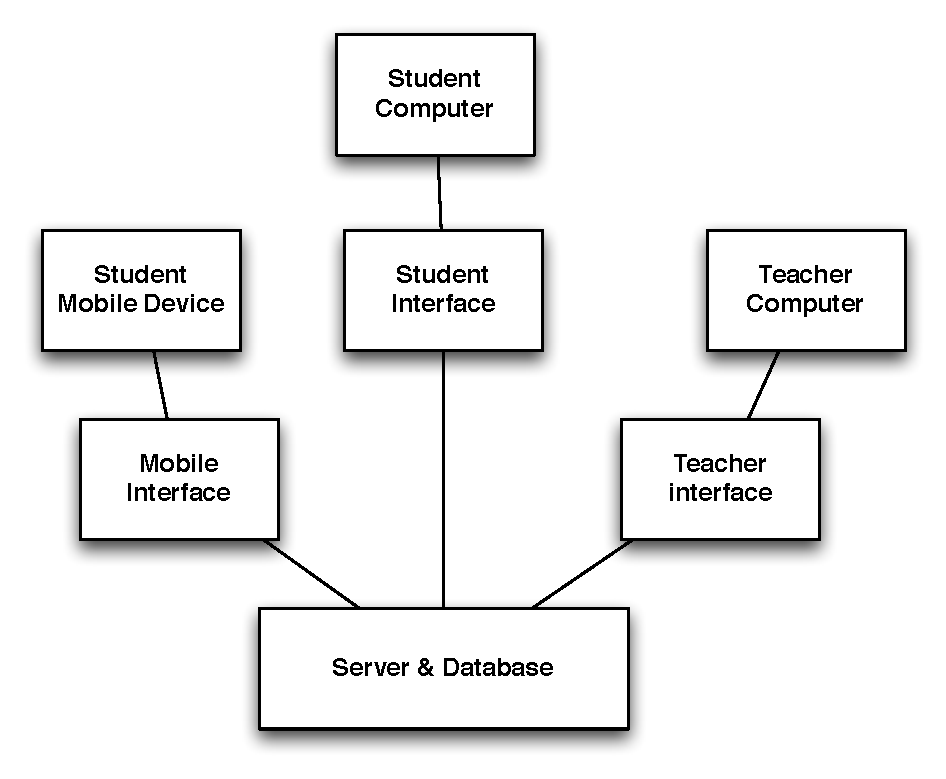
\includegraphics{systemdiagram.pdf} % requires the graphicx package
   \caption{System diagram}
   \label{fig:sysdiagram}
\end{figure}





\end{document}  